\subsection{Körvonal}

%50
\begin{frame}
  Körvonal (outline): az elemet a szegélyen kívülről körülöleli, kiemeli környezetéből. Rálóghat más elemekre.
  \begin{description}[m]
    \item[\texttt{outline-style}] \hfill \\ Stílus, mint \texttt{border-style}, pl. \texttt{solid}, \texttt{dotted}, \texttt{double}, \dots \\A többi tulajdonság beállítása \kiemel{hatástalan} a stílus megadása nélkül!
    \item[\texttt{outline-color}] Körvonal színe. Értéke lehet \texttt{invert}, ami minden háttéren látható.
    \item[\texttt{outline-width}] Szélesség CSS mértékegységekben, vagy \texttt{thin}, \texttt{medium}, \texttt{thick}.
  \end{description}
\end{frame}

%51
\begin{frame}
  Rövidítés: 
  \begin{description}[m]
    \item[\texttt{outline: outline-width outline-style outline-color}] \hfill \\ Sorrend tetszőleges, bármelyik érték elhagyható.
  \end{description}
  \vfill
  \begin{description}[m]
    \item[\texttt{outline-offset}] \hfill \\ A körvonal távolsága a szegélytől. Ez a terület áttetsző.
  \end{description}
\end{frame}

%52
\begin{frame}
  \scriptsize
  \begin{exampleblock}{\textattachfile{korvonal.html}{korvonal.html}}
    \fontsize{7}{8} \selectfont
    \lstinputlisting[style=HTML,linerange={7-12},numbers=left,firstnumber=7]{korvonal.html}
    \lstinputlisting[style=HTML,linerange={20-23},numbers=left,firstnumber=20]{korvonal.html}
  \end{exampleblock}
  \begin{center}
    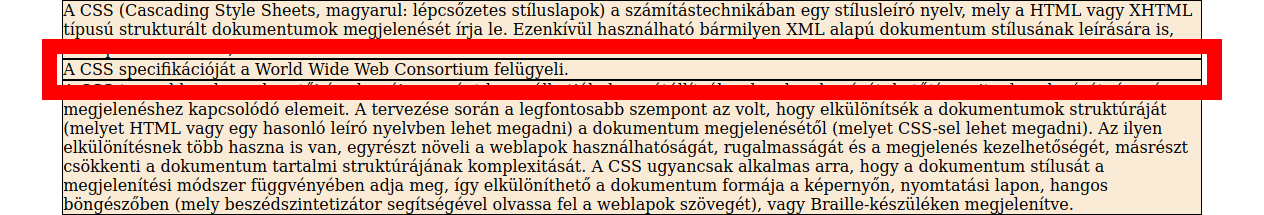
\includegraphics[width=0.9\textwidth]{korvonal.png}
  \end{center}
\end{frame}
